\documentclass[fleqn,11pt]{jreport}
\usepackage{mysty}
\usepackage[dvipdfmx]{graphicx}
\usepackage{subfigure}
\usepackage{siunitx}

\begin{document}
\baselineskip 21.5pt

\begin{titlepage}
\vspace*{3cm}
\begin{center}
{\Large\gt 東京都市大学メディア情報学部}\\
\vspace*{0.5cm}
{\Large\bf 2020年度卒業研究}\\
\vspace{1.5cm}

% 論文タイトルが1行の場合
{\huge\bf 計測不能な歩行に対応する歩数計測法の考案}\\

% 論文タイトルが2行の場合
%{\huge\bf 都市計画用住民データ推定における}\\
%\vspace{0.5cm}
%{\huge\bf 適合度算出手法の改良}\\

\vspace{9cm}
{\Large メディア情報学部 情報システム学科 1772075}\\
{\Large 松阪 僚子}\\
\vspace*{0.5cm}
{\Large 指導教員 大谷紀子 教授}\\
\end{center}
\end{titlepage}

\pagenumbering{roman}
\tableofcontents
\cleardoublepage

\pagenumbering{arabic}
% 本文のファイルを以下に列挙する
\chapter{はじめに}
主要な日常生活動作のひとつとして歩行は重要である.高齢者や片麻痺患者にとってスムーズな歩行はQOLの向上へと繋がるので,歩行の訓練は大切である.また,訓練のモチベーション維持や介護者の負担軽減など,効果的な訓練を実施するために,正確な歩数を簡便に取得できることが望ましい.

一般に歩数の測定には歩数計が用いられている.近年では,スマートフォンに加速度センサが内蔵されており,従来の歩数計の機能がアプリケーションとして実現されている.一般的に,従来の歩数計では,加速度センサを通して3軸加速度信号を取得し,地磁気センサにより検知したデバイスの傾きを補正して歩数計測に利用する.歩行と環境ノイズを区別するための閾値を設定し,設定した閾値を超えた加速度信号の回数を歩数とする.しかし,高齢者や片麻痺患者,杖歩行者など歩行速度が遅い場合や歩行リズムが不規則である場合には,歩行時の加速度が環境ノイズと区別するための閾値を超えない,もしくは歩き始めの検出が不能なため正しい歩数を取得できない.

本研究では主に前者の問題に着目し,従来の歩数計では正確な測定が不能であったケースも含めて,多くの人が精度良く測定できるようにすることを目的とし,新たな歩数計測法を提案する.


% 図はこんな風に入れます.

% \begin{figure}[tbhp]
% \begin{center}
% \includegraphics[scale=0.95]{image/se.eps}
% \caption{共生進化における2つの集団}
% \label{fig:02se}
% \end{center}
% \end{figure}

% 図番号は図\ref{fig:02se}のように参照します.
 %チョロチョロっと
\chapter{��s����}

���݁C�l�̊����ɑ������y�Ȃ�������������V�X�e���̌������i�߂��Ă���D�{�͂ł͑�J��̌���\cite{otani14}�ɂ‚��Đ�������D

�y�Ȃ𐶐�����菇�Ƃ��āC���[�U�Ɋ����y�Ȃ𒮂����C���ꂼ��̊y�Ȃ�]��������D�]�����ʂƊ����y�Ȃ̃f�[�^�Ɋ�Â��A�[�_���v���O���~���O��p���āC�g�g�\���C���`�[�t�C�a���i�s�̊������f�����l������D���Ɋe�������f���Ɋ�Â��i���v�Z�A���S���Y���ɂ���Ċy�Ȃ𐶐�����D

�����y�Ȃ̃f�[�^�ɂ́C�L�[�CBPM�C�����f�B�̊e���̉����Ɖ����C�a���i�s�̊e�a���̃R�[�h�l�[���Ɖ������܂܂�Ă���D�}\ref{fig:mu}�Ɏ������y���̃����f�B�̃f�[�^��\\ref{tab:exmelo}�C�a���i�s�̃f�[�^��\\ref{tab:excode}�Ɏ����D�����f�B�̃f�[�^�ɂ����āC�I�N�^�[�u�͒����̃I�N�^�[�u��5�Ƃ��ĕ\�����C�����̒l��4����1���̒�����1�Ƃ���D�a���̃f�[�^�̉�����1���̒�����1�Ƃ���D
���s�̃V�X�e�����p����y�ȃf�[�^�͂��ׂĎ��Ƃœ��͂���Ă���D���������đ����̊y�Ȃ�I�����Ƃ��Ē񎦂��邽�߂ɂ͖c��ȍ�Ƃ�K�v�Ƃ����肪����D


\begin{figure}[tbhp]
\begin{center}
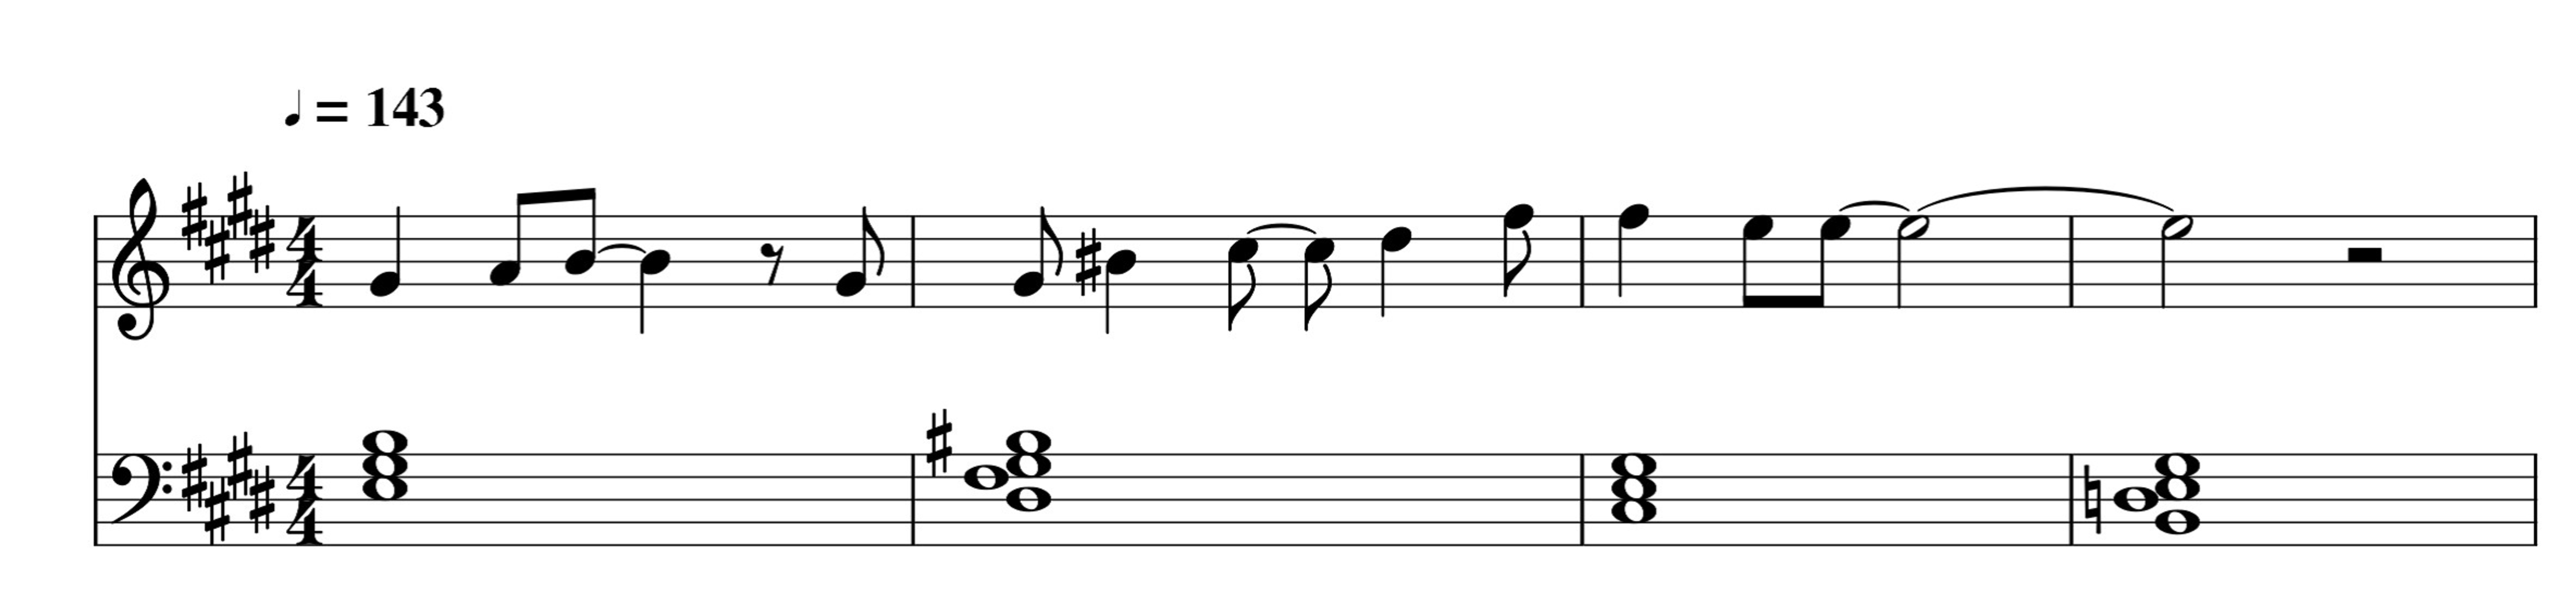
\includegraphics[scale=0.15]{image/exmu.eps}
\caption{�f�[�^��̊y��}
\label{fig:mu}
\end{center}
\end{figure}

\begin{table}[tbp]
\begin{center}
\caption{�����f�B�̃f�[�^��}
\label{tab:exmelo}
\begin{tabular}{|c|c|c|} \hline
�I�N�^�[�u&����&����\\ \hline
5&G\#&4\\ \hline
5&A&2\\ \hline
5&B&6\\ \hline
$-1$&rest&2\\ \hline
5&G\#&2\\ \hline
5&G\#&2\\ \hline
5&B\#&4\\ \hline
6&C\#&4\\ \hline
6&D\#&4\\ \hline
6&F\#&2\\ \hline
6&F\#&4\\ \hline
6&E&2\\ \hline
6&E&18\\ \hline
$-1$&rest&8\\ \hline
\end{tabular}
\end{center}
\end{table}

\begin{table}[tbp]
\begin{center}
\caption{�a���i�s�̃f�[�^��}
\label{tab:excode}
\begin{tabular}{|c|c|c|} \hline
���[�g&�^�C�v&���� \\ \hline
E&&4\\ \hline
G\#&7&4\\ \hline
C\#&m&4\\ \hline
E&7&4\\ \hline
\end{tabular}
\end{center}
\end{table}


 %背景
\chapter{�`�a�b�V�X�e��}
����������������������������������������������������������������������������������������������������������������������������������������������������������������������������������������������������������������������������������������������������������������������������������������������

\section{����������}
����������������������������������������������������������������������������������������������������������������������������������������������������������������������������������������������������������������������������������������������������������������������������������������������


\section{����������}
����������������������������������������������������������������������������������������������������������������������������������������������������������������������������������������������������������������������������������������������������������������������������������������������

 %歩数計測法概要
\chapter{システム構成}
本章では、本研究で構築したProgressive Houseのメロディ生成支援システムについて説明する。

\section{メロディルールの獲得}
メロディルールとは,メロディ生成においてProgressive Houseらしさを表現する際に使用するメロディの特徴データである.音高差分データ,リズムデータ,メロディ変異データ,およびメロディ繰り返し回数データで構成され,有名なProgressive Houseの既存曲のサビ部分冒頭16小節のみを学習データとして獲得される.
\subsection{音高差分データ}
音高差分データとは,学習データに含まれる各音とキーの音高の差を表した数値である.
\subsection{リズムデータ}
リズムデータとは,学習データに含まれる各音の音価を表した数値である.
\subsection{メロディ変異データ}
変異データとは,学習データのメロディを繰り返し回数分に分割し,それぞれの音数や音高,リズムを比較して算出した差分である.
\subsection{メロディ繰り返しデータ}
繰り返し回数データとは,学習データのメロディ内における同じメロディの繰り返し回数である.繰り返し回数は,音高とリズムの類似度から算出する.はじめにメロディを4小節ごとに分割し,1小節目のメロディと,2,3,4小節目のメロディを比較し,一致している割合を類似度として算出する.類似度が60\%以上の場合,繰り返し回数は4回とする.60\%未満の場合は,学習データのメロディの前半8小節と後半8小節の類似度を算出する.60\%以上一致している場合、繰り返し回数は2回とする.すべてに該当しないメロディの繰り返し回数は0回とする.

\section{メロディの生成}
メロディ生成手順を示す。
概要を参考に箇条書きで書く


\section{メロディ評価部}
あああああああああああああああああああああああああああああああああああああああああああああああああああああああああああああああああああああああああああああああああああああああああああああああああああああああああああああああああああああああああああああああああああああああああああああああ

 %粒子群最適化による歩数計測
\chapter{考察}
楽曲Dでは,リズム感の良さと伴奏の合致度について提案手法より(c),(d)の方が評価値の平均が高い.
自由記述では「フレーズの切れ目にそった伴奏に良い評価をする傾向があった」という意見が挙げられた.
楽曲Dには,1小節あたりの和音の移り変わりが多い特徴がある.現状ではルール適用の際,フレーズの切れ目を考慮していない.フレーズの切れ目では,音高の変化が大きい方がメロディに合うと考えられる.

%「伴奏とメロディの音域が離れすぎているものは悪く評価する影響があった」という意見があげられた.

提案手法において,楽曲Eではリズム感の良さについて適用前の音源より高い評価が得られていることから,リズム感をもった楽曲を生成できているといえる.
しかし,伴奏の適合度については2.1と他の音源に比べ大幅に低い.自由記述では「分散の伴奏の時にメロディと音がぶつかる」との指摘があった.
提案手法では,音の衝突を回避することを考慮していない.メロディと伴奏部の音の衝突は評価を下げると考えられる.

楽曲Lでは,提案手法よりも他の分散和音を適用した音源の方がリズム感の良さの評価が高い.
自由記述では「伴奏によって雰囲気が変わる」という意見が複数挙げられた.
伴奏が楽曲全体の雰囲気を変え,評価に影響を与えたと考えられる.

適用前の音源において,楽曲Jではリズム感の良さについて他の音源より評価が低いので,リズム感に欠けているといえる.
しかし楽曲Jでは,伴奏の適合度について平均が4.2と適用前の音源における評価値が提案手法を上回った.
自由記述では「遅めのメロディに対して細かく刻むような伴奏の楽曲は良い印象を抱かなかった」という意見が挙がった.
曲Mのメロディは1小節あたりの音数が少ない.現状では伴奏部を生成する際,音数を考慮していない.
メロディの音数が少ない部分では,伴奏部の音数が多いと,メロディのリズムを阻害すると考えられる.
 %自己相関による歩数計測
\chapter{考察}
あああああああああああああああああああああああああああああああああああああああああああああああああああああああああああああああああああああああああああああああああああああああああああああああああああああああああああああああああああああああああああああああああああああああああああああああ
 %動的閾値による歩数計測
\chapter{�l�@}
�]�������̌��ʂ���C�{�V�X�e���̓��[�U�̕]�������Ɋy�Ȃ��J��Ԃ��������C�ŏI�o�͂Ń��[�U�̖�������y�Ȃ�񎦂��邱�Ƃ��”\�ł���Ƃ킩�������ƂŁC�{�V�X�e���̗L�p�����������Ƃ�����D
�������C�y�Ȃ̕ω������Ȃ����[�U�������܂łɖO����”\��������C�����㐶�����J��Ԃ��Ă��y�Ȃɖ��m�ȕω��������K�v������ƍl������D���P��Ƃ��āC���F�̂Ɋy��̏������������㐶���ʼn��F�ɕω��������邱�Ƃ���������D�܂��C�]�����ꂽ6�Ȃ̂����ɒ[�ɕ]���̒Ⴂ�y�Ȃ���������C��������6�Ȃ����ׂĎ��Ă����肷��ꍇ�C6�Ȃ̂�����1�Ȃ𖳍�ׂɐ��������ȂɕύX���邱�Ƃ���������D
�O���̌����ɂ‚��Ă̋L�q���y�Ȃ̏��Ȃ��ω��ɂ����̂��������C�y�Ȃ̕ω������Ȃ����Ƃɂ�胆�[�U�͔�r�̂��߂ɌJ��Ԃ��y�Ȃ𒮂��Ɛ��������D���������Ĉȏ�̉��P�Ăɂ���ẮC������ׂ�񐔂��������C�ŏI�o�͂̒񎦂܂ł̎��Ԃ�Z�k�ł���ƍl������D

�܂��C�C���^�t�F�[�X�̕]���ɂ��C�C���^�t�F�[�X���g���Â炳�ł̃��[�U�ւ̈��e���͂Ȃ������Ɛ����ł���D�e�p�[�g�̉��ʂɊւ��ẮC�ቹ��ł���x�[�X���C���̈�ۂ����ꂽ���C�����ɗp�����C���z���̐��\�����ƍl������D %評価実験
\chapter{考察}
「歩行は周期的な信号であるので,個人に合わせた閾値をはじめに設定することで正確に歩数を測定できるようになる」という仮説を立てたが,被験者の体調によって歩幅や歩行速度が異なるために歩行を一定の閾値によって測定することは困難であると考えられる.粒子群最適化による歩数計測法については前述の理由に加えて,閾値算出の実行時間が平均約16時間かかるため,実用性に乏しいと考えられる.

自己相関関数による歩数計測法についても,歩数計としては高精度とならなかった.自己相関関数は感度が高く,ポケットにiPhoneを入れる際の振動など,ノイズの波形が歩行中の信号と偶然類似している場合にも歩数と数えていることが原因であると考えられる.

動的閾値による歩数計測法は本研究において最も良い結果を記録した.従来の歩数計においても使用されることのある計測法であるが,動的閾値の算出窓長を変更することで精度が変わる.本研究では評価実験に用いたデータとは別のデータにおいて窓長90サンプルが最も良い結果が出たため90サンプルを窓長として使用しているが,個々人に対応するために例えば「自己相関関数を算出する過程で得られる信号の周期を動的閾値の窓長とする」など工夫する必要があると考えられる.

今後の課題として,歩き始めの検出についての検討を重ねる必要があることが挙げられる.しかしながら,被験者のデータにおいて,従来の歩数計では計測が不能であったが,本研究で提案した3つの歩数計測法すべてで歩行を確認することができた.本手法を用いることで,従来の歩数計で測定不能であった対象者の正確な歩数計測が可能となり,より効果的な歩行訓練の提供,モチベーションの向上,および健康増進へ繋がると期待される.
 %考察
\chapter{おわりに}
本研究は,従来の歩数計では正確な測定が不能であった高齢者や片麻痺患者を対象とし,歩数計の測定精度を向上させるための新たな歩数計測法を提案することを目的とした.提案する手法は,3軸加速度信号から粒子群最適化を用いて閾値を算出し,得た閾値を基に歩数を数える方法,自己相関関数を用いて周期性の有無を確認し歩数を数える方法,動的閾値を用いて歩数を数える方法の3つがある.
杖歩行の片麻痺患者において測定精度を検討したところ,従来の歩数計ではすべての歩行について測定不能であったことに対し,本研究で提案する手法では粒子群最適化を用いた歩数計測法,自己相関関数を用いた歩数計測法,動的閾値を用いた歩数計測法それぞれについて誤差は71\%,29\%,14\%であり,歩行を確認することができた.本研究で提案する手法は,杖歩行時のみならず,歩行速度が遅い,または下肢機能障害を持つなど従来の歩数計で困難であった高齢者の歩数検出率を高めることが可能であり,より効果的な歩行訓練の提供,モチベーションの向上,および健康増進へ繋がると期待される. %おわりに

\chapter*{謝 辞}
\markboth{謝 辞}{謝 辞}
\addcontentsline{toc}{chapter}{謝 辞}
本研究を進めるにあたり,ご指導下さった大谷紀子教授に感謝致します.
また,評価実験のアンケートに協力頂いた皆様,
および本研究に関するアドバイスをしていただいた皆様に感謝の意を表します.


\markboth{参考文献}{参考文献}
\bibliographystyle{jsai}
%\bibliographystyle{plain}
\bibliography{mybib}



\appendix
% 付録のファイルを以下に列挙する
\chapter{Progressive Houseメロディ生成システムの画面}
被験者への説明に使用した使い方説明画面を図A.1に,初期生成のための情報入力画面を図A.2に,メロディ評価画面を図A.2に示す.

\vskip\baselineskip
\begin{figure}[htbp]
	\begin{center}
		\includegraphics[width=15cm]{image/mainDisplay1.png}
		\caption{使い方説明画面}
	\end{center}
\end{figure}

\begin{figure}[htbp]
	\begin{center}
		\includegraphics[width=15cm]{image/mainDisplay2.png}
		\caption{情報入力画面}
	\end{center}
\end{figure}

\begin{figure}[htbp]
	\begin{center}
		\includegraphics[scale=0.35]{image/subDisplay.png}
		\caption{メロディ評価画面}
	\end{center}
\end{figure}

\end{document}
